\section{Expectation Maximization Algorithm}

Die geforderte Funktion wurde wie in der Angabe angegeben implementiert. Für die Normalverteilung wurde die Funktion \texttt{mvnpdf} verwendet. Die Funktion \texttt{EM} ist im Anhang zu finden, so wie das Skript \texttt{hw6\_1.m}, welches die Berechnungen durchführt.

Abbildung \ref{fig:6_1_EM_classification} zeigt die Klassifikation der Daten nach einem Durchlauf bis Konvergenz festgestellt wurde\footnote{sobald die Differenz zum vorigen Wert der log-Likelihood eine Grenze unterschreitet}. Man erkennt, dass die erkannten Gaußverteilungen recht gut mit den tatsächlichen Punktmengen zusammenpassen. Bei jedem Durchlauf erhält man natürlich ein etwas anderes Ergebnis.

\begin{figure}[h!]
  \centering
	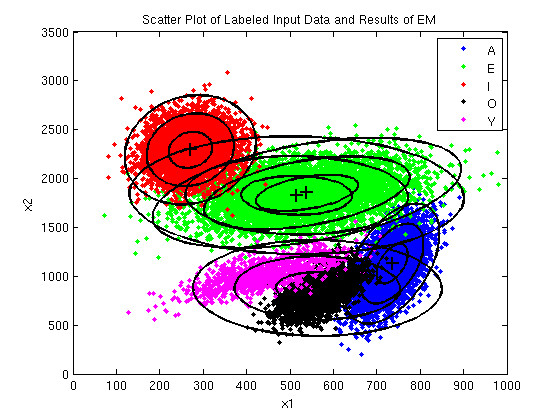
\includegraphics[width=0.8\textwidth]{./figures/6_1_EM_classification.png}
	\caption{Ergebnis der Klassifikation mit EM-Algorithmus}
	\label{fig:6_1_EM_classification}
\end{figure}

Wie auf der Abbildung ersichtlich funktioniert die Klassifikation mit $M=5$ Komponenten recht gut. Bei einer anderen Anzahl an Komponenten werden Punktwolken teilweise mehrfach erkannt bzw. nicht erkannt.

Die Wahl der Anfangsparameter hat natürlich Auswirkungen auf das Ergebnis. Bei einer schlechten Wahl kann es dazu kommen, dass lokale Maxima erreicht werden. Bei extrem schlechter Parameterwahl kann es auch zu Fehlern in der Ausführung kommen, da z.B. eines der $N_m = 0$ ist (kein einziger Punkt dieser Komponente zugeordnet) und dadurch eine Division durch Null auftritt.

Unsere Implementation wählt für $\mu_m$ zufällige Werte in dem Bereich, in dem sich die Werte des Datensatzes befinden. Für $\Sigma_m$ werden recht große Kovarianzen gewählt, um einen möglichst großen Bereich abzudecken. Die $\alpha_m$ wurden mit 1 initialisiert. $\mu_m$ und $\alpha_m$ nähern sich dann dem Zielwert an, $\Sigma_m$ schrumpft auf den richtigen Wert.

Abbildung \ref{fig:6_1_EM_performance} zeigt die log-Likelihood über die Iterationen. Man erkennt, dass diese anfangs recht schnell auf größere Werte steigt, aber dann sich langsam noch bis zur Grenze weiterentwickelt. Auch diese Entwicklung sieht bei jedem Durchlauf anders aus.

\begin{figure}[h!]
  \centering
	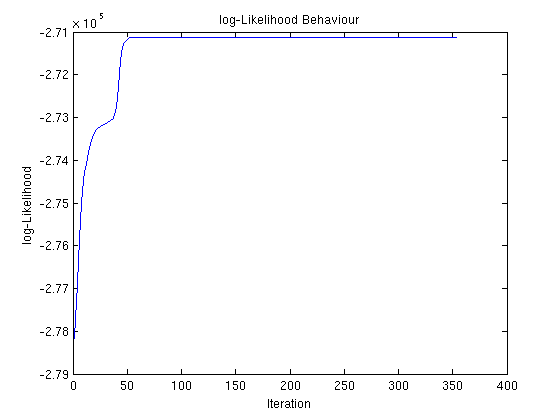
\includegraphics[width=0.8\textwidth]{./figures/6_1_EM_perf.png}
	\caption{Performance der Klassifikation mit EM-Algorithmus}
	\label{fig:6_1_EM_performance}
\end{figure}

Die Funktion \texttt{EM\_diagonal}, welche den EM-Algorithmus für diagonale Covarianzmatrizen durchführt, ist ebenfalls im Anhang zu finden. Im Gegensatz zur Version mit voll besetzten Covarianzmatrizen ist hier die Berechnung etwas einfacher, da nur der Differenzvektor von $X$ und $\mu$ quadriert und aufsummiert werden muss. Statt die gesamte Matrix zu speichern wird nur ein Vektor mit den Diagonalelementen gespeichert.

Abbildung \ref{fig:6_1_EM_classification_diag} zeigt die Klassifikation mit dem EM-Algorithmus mit diagonalen Covarianzmatrizen. Dadurch, dass die Elemente außerhalb der Hauptdiagonale 0 sind, werden die Dimensionen als unkorreliert angenommen. Dadurch sind die Varianzen der Gaußverteilungen immer achsparallel, deshalb liegen die Ellipsen der Varianzen nicht mehr beliebig in der Grafik, sondern entweder waagrecht, senkrecht oder als Kreis. Korrelierte Dimensionen können dadurch nicht so gut klassifiziert werden als mit beliebigen Covarianzmatrizen.

\begin{figure}[h!]
  \centering
	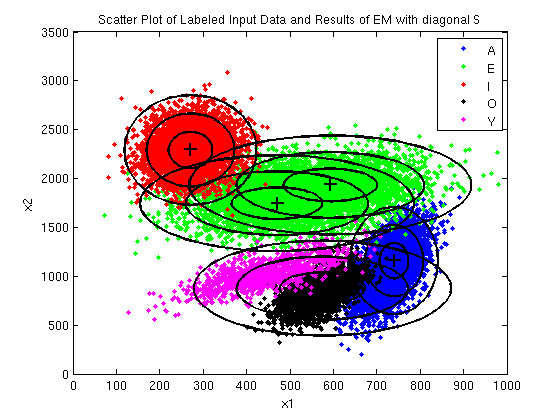
\includegraphics[width=0.8\textwidth]{./figures/6_1_EM_classification_diag.png}
	\caption{Ergebnis der Klassifikation mit EM-Algorithmus mit diagonalen Covarianzmatrizen}
	\label{fig:6_1_EM_classification_diag}
\end{figure}

Abbildung \ref{fig:6_1_EM_performance_diag} zeigt die Entwicklung der log-Likelihood bei der Variante mit diagonalen Covarianzmatrizen. Die Entwicklung sieht ähnlich aus, dauert aber länger.

\begin{figure}[h!]
  \centering
	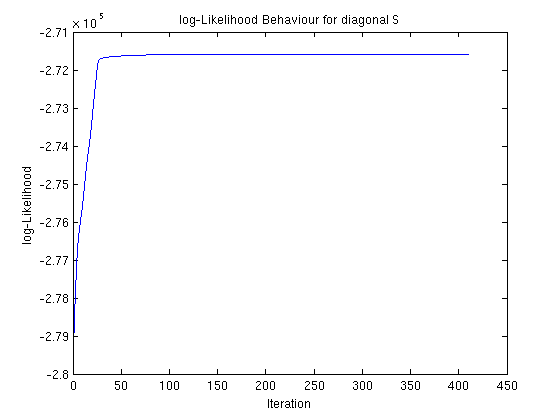
\includegraphics[width=0.8\textwidth]{./figures/6_1_EM_perf_diag.png}
	\caption{Performance der Klassifikation mit EM-Algorithmus mit diagonalen Covarianzmatrizen}
	\label{fig:6_1_EM_performance_diag}
\end{figure}

Abbildung \ref{fig:6_1_EM_soft_classification} zeigt die Ergebnisse der Soft-Classification im Expectation-Step nach der letzten Iteration.

\begin{figure}[h!]
  \centering
	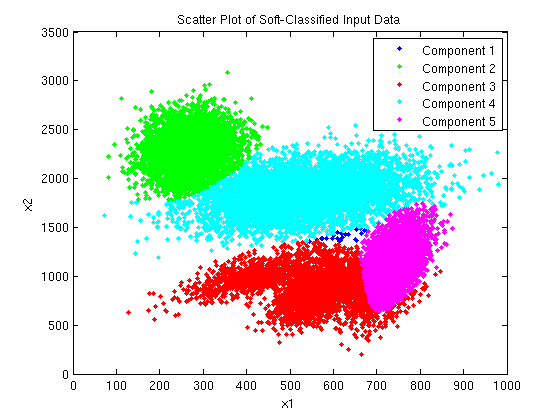
\includegraphics[width=0.8\textwidth]{./figures/6_1_EM_soft_classification.png}
	\caption{Ergebnis der Soft-Classification mit EM-Algorithmus}
	\label{fig:6_1_EM_soft_classification}
\end{figure}
